\scanpage{24}
\mspage{12}
\figure{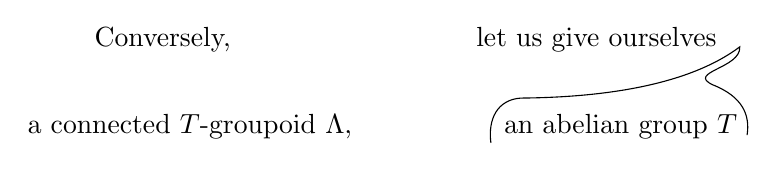
\begin{tikzpicture}[x=1cm,y=1cm]
\node[anchor=base west,inner sep=0pt,text width=7.9cm] at (0,1.10) {Conversely,\hfill let us give ourselves};
\node[anchor=base west,inner sep=0pt] at (-0.85,0) {a \deleted{\unsure{connected}} $T$-groupoid $\Lambda$,};
\node[anchor=base west,inner sep=0pt] (abelianaddition) at (5.20,0) {\inserted{an abelian group $T$}};
\draw[thin] (5.04,-0.12) .. controls (5.00,0.18) and (5.12,0.43) .. (5.42,0.45)
 .. controls (6.60,0.46) and (7.60,0.65) .. (8.20,1.10)
 .. controls (8.22,0.83) and ([xshift=-0.65cm,yshift=0.78cm]abelianaddition.base east) .. ([xshift=-0.32cm,yshift=0.62cm]abelianaddition.base east)
 .. controls ([xshift=0.06cm,yshift=0.47cm]abelianaddition.base east) and ([xshift=0.16cm,yshift=0.24cm]abelianaddition.base east) .. ([xshift=0.12cm,yshift=-0.02cm]abelianaddition.base east);
\end{tikzpicture}} an action of $\unsure{\mathcal E|\Sigma}$ on $(T,\Lambda)$, and a homomorphism of groupoids
\diagram{\begin{tikzcd}[ampersand replacement=\&]
\Lambda \arrow[r,"\text{\uuline{faithful} functor}"] \& \begin{gathered}\text{groupoid \unsure{with|:} a single object}\\\text{of the universal coverings of}\\\Pi\text{ equal \unsure{to|:} }\widetilde\Pi\\\text{whose automorphisms are }\pi\end{gathered}
\end{tikzcd}}
compatible with action of $\unsure{\mathcal E|\Sigma}$.
Let $\unsure{\tau|\mathcal T}=\operatorname{Ob}\Lambda$ [thus $\unsure{\tau|\mathcal T}$ is an $\unsure{\mathcal E|\Sigma}$ set,] and for $\forall\,t,t'\in\unsure{\tau|\mathcal T}$, we have an \uline{injective} homomorphism
\diagram{\begin{tikzcd}[ampersand replacement=\&]
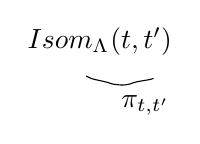
\begin{tikzpicture}[baseline=(isomop.base),x=1cm,y=1cm]
\node[anchor=base west,inner sep=0pt] (isomop) at (0,0) {$\operatorname{Isom}_\Lambda$};
\node[anchor=base west,inner sep=0pt] (isomargs) at (isomop.base east) {$(t,t')$};
\draw[thin] ([xshift=-0.30cm,yshift=-0.35cm]isomop.base east)
 .. controls ([xshift=-0.23cm,yshift=-0.40cm]isomop.base east) and ([xshift=-0.12cm,yshift=-0.40cm]isomop.base east) .. ([yshift=-0.44cm]isomop.base east)
 .. controls ([xshift=0.08cm,yshift=-0.47cm]isomop.base east) and ([xshift=0.20cm,yshift=-0.47cm]isomop.base east) .. ([xshift=0.26cm,yshift=-0.45cm]isomop.base east)
 .. controls ([xshift=-0.45cm,yshift=-0.41cm]isomargs.base east) and ([xshift=-0.32cm,yshift=-0.41cm]isomargs.base east) .. ([xshift=-0.24cm,yshift=-0.38cm]isomargs.base east);
\node[anchor=base west,inner sep=0pt] at ([xshift=0.14cm,yshift=-0.75cm]isomop.base east) {$\pi_{t,t'}$};
\end{tikzpicture} \& \unsure{\hookrightarrow|\lhook\joinrel\relbar} \& \pi
\end{tikzcd}}
compatible with composition of isomorphisms.

We have expressed the datum of a faithful functor from a groupoid $\Lambda$ into $\langle\pi\rangle$ \deleted{But \unsure{we}} [one must give oneself a family of subgroups $(\pi_t)_{t\in\unsure{\tau|\mathcal T}}$ of $\pi$ and of empty sets or bitorsors under the $\pi_{t'},\pi_t\ldots$] We are now going to introduce the actions of
\mspage{23}
